\subsection{Polimorfismo}

Polimorfismo é a capacidade que dois ou mais objetos de uma classe-filha tem  de
responder a mensagens de diferentes formas
\cite{php5ConceitosProgramacaoEIntegracaoComBancoDeDados}.

Ou seja, polimorfismo é a possibilidade que um objeto tem de alterar o
comportamento de um objeto com base em uma classe especialista, sendo assim,
são métodos que fornecem resultados distintos  de acordo com a subclasse
\cite{php5ConceitosProgramacaoEIntegracaoComBancoDeDados}. Desta forma, quem
chama o método não precisa distingui-lo.

A seguir, será apresentada a atribuição deste conceito no processo de aceleração
de um veículo. Por conta disto, imagine o exemplo a seguir: dentre os comandos
disponíveis em um veículo, tem-se o acelerador que fornece uma interface
encapsulando a forma de como um motor realiza a aceleração. Suponha que
deseja-se acelerar dois veículos diferentes, o primeiro veículo trata-se de um 
carro popular com motor 1.0, enquanto que o outro veículo é um esportivo, que
neste caso, possui um motor 2.0. Então, ambos os veículos possuem a mesma
interface de comunicação: o pedal acelerador, que permite ao condutor se
locomover de maneira mais rápida.

Note que, quando o condutor acelerar o carro popular este deverá ter aceleração
mais lenta se comparado ao esportivo, na prática é disto que se trata o polimorfismo.

Voltando-se para o paradigma da orientação a objetos seria possível existir uma
classe generalista chamada \textit{Carro} que seria responsável em definir um
meio padronizado para realizar a aceleração de um veículo. E, com base nesta
classe, criar duas outras classes especialistas, sendo que, poderiam ser
nomeadas como: \textit{CarroPopular} e \textit{CarroEsportivo}.

Na Figura \ref{fig:polimorfismo} será apresentada a implementação destes conceitos
utilizando a linguagem de programação \acs{PHP}.

\begin{figure}[h!tb]
	\caption{Polimorfismo com implementação na linguagem PHP}
	\label{fig:polimorfismo}

	\centering
	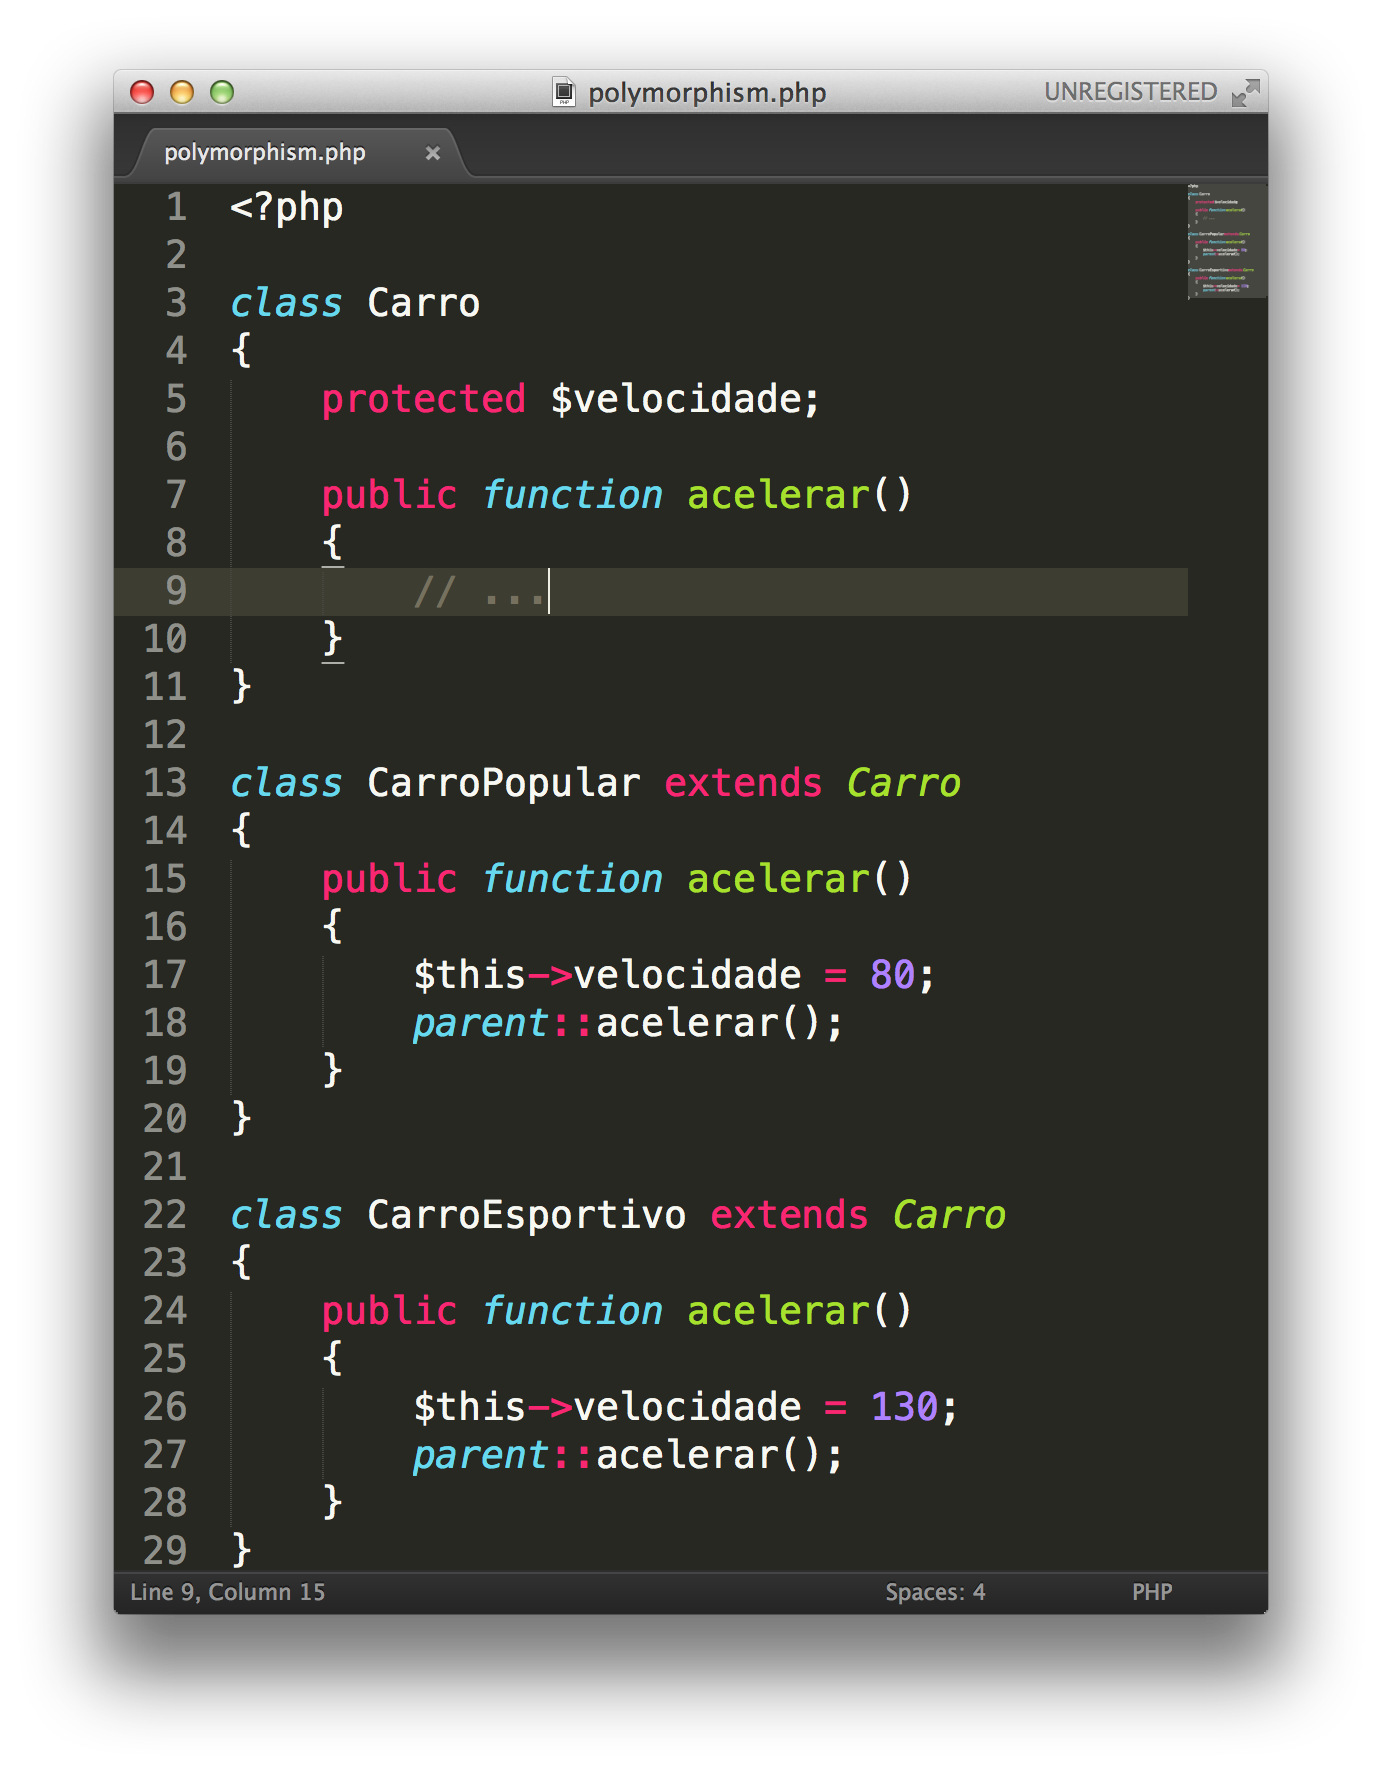
\includegraphics[width=0.75\textwidth]{images/polymorphism.png}

	\centering
	\footnotesize Fonte: \fonteOAutor
\end{figure}

\FloatBarrier 	% Este comando impede que as imagens
				% flutuem a partir deste ponto no seu documento

A seguir, apresenta-se em detalhes as linhas de código exibidas na Figura
\ref{fig:polimorfismo}:

\begin{alineas}
    \item linha 3: define-se a existência da classe \textit{Carro};
    \item linha 4: tem-se a declaração do método \textit{acelerar} que trata de
    uma forma padrão de acelerar qualquer veículo;
    \item linha 13: define-se a classe \textit{CarroPopular}, sendo que ela
    herda todas as características e funcionalidades da classe \textit{Carro};
    \item linha 15: reescreve-se o método \textit{acelerar} que foi definido na
    classe \textit{Carro}, pois um carro popular acelera neste caso a uma
    velocidade de oitenta quilômetros por hora;
    \item linha 22: define-se a classe \textit{CarroEsportivo}, que, da mesma
    maneira que a classe \textit{CarroPopular}, herda as propriedades e métodos
    que foram definidos na classe pai \textit{Carro};
    \item linha 24: redefine-se o método \textit{acelerar}, pois um carro
    esportivo acelera a uma velocidade constante de cento e trinta quilômetros
    por hora (neste caso).
\end{alineas}

Conforme foi visto neste capítulo, ambos os veículos aceleram, entretanto o
carro esportivo tem um desempenho melhor do que o carro popular, entretanto, a
modelagem permite reusar a classe carro e definir apenas as características
pertinentes a ambos os veículos, sendo assim, os objetos que chamarem esta
classe não entendem como a implementação acontece, mas realmente aceleram de
maneira correspondente ao tipo de veículo.

A seguir será apresentado o conceito de encapsulamento, que permite esconder do
escopo público os dados sensíveis, tais como as propriedades de uma classe.
